% AMS dept HW template example
% v0.04 by Eric J. Malm, 10 Mar 2005
\documentclass[11pt,a4paper,boxed]{caspset}

% set 1-inch margins in the document
\usepackage[left=1in,right=1in,top=1.2in,bottom=1in]{geometry}
\usepackage{lastpage}
% include this if you want to import graphics files with /includegraphics
\usepackage{graphicx}
\usepackage{amsmath,amsfonts,amsthm,amssymb}
\usepackage{setspace}
\usepackage{fancyhdr}
\usepackage{lastpage}
\usepackage{extramarks}
\usepackage{chngpage}
\usepackage{soul}
\usepackage[usenames,dvipsnames]{color}
\usepackage{graphicx,float,wrapfig}
\usepackage{ifthen}
\usepackage{listings}
\usepackage{courier}
\usepackage{multimedia}
\usepackage[toc,page,title,titletoc,header]{appendix}
\usepackage{indentfirst}
%%%%%%%%%%%%%%%%%%%%%%%%%%%%%%%%%%%%%%%%%%%%%%%%%%%%%%
\usepackage{xeCJK}
%\usepackage{fontspec}
\setCJKmainfont[BoldFont=simhei.ttf]{simsun.ttf}
%\setCJKsansfont{simhei.ttf}
%\setCJKmonofont{simfang.ttf}

%\setCJKmainfont{Adobe Song Std}
%\setCJKmainfont[BoldFont=Adobe Heiti Std]{Adobe Song Std}
%%%%%%%%%%%%%%%%%%%%%%%%%%%%%%%%%%%%%%%%%%%%%%%%%%%%%%

\graphicspath{{figures/}}
% Homework Specific Information
\renewcommand\refname{\bf 参考文献}
\renewcommand\contentsname{\bf 目 \ \ \ 录}
\renewcommand\figurename{\bf 图}
\renewcommand\tablename{\bf 表}
\renewcommand\appendixname{\bf 附录}
\renewcommand{\appendixpagename}{附录}

\newtheorem{dingyi}{\bf 定义~}[section]
\newtheorem{dingli}{\bf 定理~}[section]
\newtheorem{yinli}[dingli]{\bf 引理~}
\newtheorem{tuilun}[dingli]{\bf 推论~}
\newtheorem{mingti}[dingli]{\bf 命题~}


\newcommand{\hmwkTitle}{现代物理问题的计算机模拟}
\newcommand{\hmwkSubTitle}{} % No subtitle, so this will be excluded
\newcommand{\hmwkDueDate}{10/02/2011}
\newcommand{\hmwkClass}{物理学院}
\newcommand{\hmwkClassTime}{Thu/Fri{~}8:00}
\newcommand{\hmwkClassInstructor}{周昕}
\newcommand{\hmwkAuthorName}{周吕文}


%% Setup the header and footer
\pagestyle{fancy}                                                       %
\lhead{\hmwkAuthorName}                                                 %
\chead{\hmwkClass\ (\hmwkClassInstructor): \hmwkTitle}  %
\rhead{第\ \thepage\ 页,{~} 共\ \protect\pageref{LastPage} 页}          %                                %
\definecolor{DarkGreen}{rgb}{0.0,0.45,0.0}

%%%%%%%%%%%%%%%%%%%%%%%%%%%%%%%%%%%%%%%%%%%%%%%%%%%%%%%%%%%%%

\setlength{\parskip}{5pt}
%%%%%%%%%%%%%%%%%%%%%%%%%%%%%%%%%%%%%%%%%%%%%%%%%%%%%%%%%%%%%

\usepackage{palatino}
\usepackage{listings} % Gives syntax highlighting for python code.
\usepackage{color} % Used for syntax highlighting.
\usepackage{textcomp} % Used for syntax highlighting.

% This gives syntax highlighting in the python environment
\renewcommand{\lstlistlistingname}{Code Listings}
\renewcommand{\lstlistingname}{Code Listing}
\definecolor{gray}{gray}{0.5}
\definecolor{key}{rgb}{0,0.5,0}
\lstnewenvironment{python}[1][]{
\lstset{
language=python,
basicstyle=\ttfamily\small,
otherkeywords={1, 2, 3, 4, 5, 6, 7, 8 ,9 , 0, -, =, +, [, ], (, ), \{, \}, :, *, !},
keywordstyle=\color{blue},
stringstyle=\color{red},
showstringspaces=false,
emph={class, pass, in, for, while, if, is, elif, else, not, and, or,
def, print, exec, break, continue, return},
emphstyle=\color{black}\bfseries,
emph={[2]True, False, None, self},
emphstyle=[2]\color{key},
emph={[3]from, import, as},
emphstyle=[3]\color{blue},
upquote=true,
morecomment=[s]{"""}{"""},
commentstyle=\color{gray}\slshape,
framexleftmargin=1mm, framextopmargin=1mm, frame=shadowbox,
rulesepcolor=\color{blue},#1
}}{}



% info for header block in upper right hand corner
\name{周吕文{~}201128000718065}
\class{物理学院{~}20110308班}
\assignment{Project \# 02}
\duedate{10/02/2011}


\begin{document}

\problemlist{\LARGE\bf 伊辛(Ising)模型的蒙特卡罗(Monte Carlo)模拟}
\section{引言}
在近现代物理学中, 相变问题是一个很前沿的课题, 在很多实际的问题
中都起到了重要的作用.
伊辛模型是最早以自旋模型研究磁性物质相变问题的模型. 1920年由德国物理学家Wilhelm Lenz和他的学生Ernst Ising提出. 在该模型中, 用离散变量来表示每个粒子的自旋状态, 这种离散变量只有两种取值可能. 这些粒子被排布于网格中, 每个粒子只与其最近邻的其它粒子相互作用.

伊辛模型虽然很简单, 却可以提供非常丰富的物理内容. 它可以用来描述晶体的磁性, 还可
以用来描述非常广泛的现象, 如合金中的有序无序转
变, 液氦到超流态的转变, 液体的冻结和蒸发, 晶格气
体,玻璃物质的性质. 伊辛模型不仅被可以用来研究物理世界, 近些年来还被广泛的用于其它领域的研究, 如森林火灾, 城市交通, 蛋白质分子
进入活性形式的折叠等.

伊辛模型提出已有近百年, 大量科学家对该模型作了深入的研究. Ising于1925年发表了一维模型求解的结果, 并证明一维情况下伊辛模型没有相变; 1936年Peierls论
证了二维或三维的伊辛模型存在着自发磁化. 1944年, Onsager给出了二维
伊辛模型的严格解, 并因此
获得了诺贝尔奖。在此之后很多人又相继发表伊辛模型的各种不同解法, 但至今没有被学术界公认的三维伊辛模型精确解.

对于二维的伊辛模型, 在理论分析上已有重要的成果, 即可以求得严格解.
但尽管如此, 并不能给出物理图像. 而三维或更高维的伊辛模型, 理论分析也似乎失效.
随着计算机的发展, 模拟成为研究高维伊辛模型的一种重要手段.
Monte-Carlo方法就是其中的一种. 它不仅可以求出模型的
解, 并且还可以给出具体的图像与涨落. 本文基于蒙特卡罗模拟方法, 对二维伊辛模型进行模拟.

\section{伊辛模型}
二维的伊辛模型是统计物理中最简单的格点系统之一, 它的能量可以用系统的一个哈密顿量来描述. 考虑一个二维方点阵,
每个格点为一个自旋, 每个自旋可能的状态$s_i\in\{-1, +1\}$. -1表是自旋向下, +1表示自旋向上. 自旋只和最相邻的其它四个自旋相互作用. 外磁场为$h$, 则任意一个自旋的能量为
\[
E_i = - J\sum_{\{s_j\}}s_is_j - hs_i
\]
则系统的总能量为
\[
H = - J\sum_{\langle i,j \rangle}s_is_j - h\sum_{i}s_i
\]
为简化模型, 便于模拟, 本文取耦合常数$J=1$, 外场$h=0$. 基于以上模型, 由统计方法可得系统的内能和比热:
\begin{equation}
U = \langle H \rangle_T
\end{equation}
\begin{equation}
C_v = \frac{\partial U}{\partial T} = \frac{\mathrm{var}(H)}{T^2}
\end{equation}
以及磁化强度和磁化率
\begin{equation}
M = \langle \sum_i s_i \rangle_T
\end{equation}
\begin{equation}
\chi = \frac{\partial B}{\partial H} = \frac{\mathrm{var}(M)}{T}
\end{equation}
其中$\mathrm{var}(H)=\langle H^2\rangle_T-\langle H \rangle_T^2$, $\mathrm{var}(M)=\langle M^2\rangle_T-\langle M \rangle_T^2$.

\section{蒙特卡罗模拟}
对于一个$L\times L$的二维伊辛模型点阵, 系统可以出现$2^{L\times L}$种可能的状态.(如果$L=10$, 可能状态总数为$2^{100}$). 模拟 需要找到某个给定温度下的平衡状态, 所谓平衡状态: 由该状态迁移为其它状态的概率与其它状态迁移到该状态的概率相同, 即
\[
P(s_i)P(s_i\rightarrow s_j) = p(s_j)P(s_j\rightarrow s_i)
\]
上式是由Metropolis (1953)提出的细致平衡条件, 统计物理中认为最终平衡态服从Boltzmann分布, 因此
\[
\frac{P(s_i\rightarrow s_j)}{P(s_j\rightarrow s_i)} = \frac{P(s_j)}{P(s_i)} = e^{-(E_j-E_i)/kT}
\Rightarrow
P(s_i\rightarrow s_j) = \frac{e^{-E_j/kT}}{e^{-E_j/kT}+ e^{-E_i/kT}} = \frac{1}{(1+e^{\Delta E_{ij}/kT})}
\]
因此, 伊辛模型的蒙特卡罗模拟可由以下步骤实现
\begin{enumerate}
\item 随机的选择一个点$(i,j)$
\item 计算位于$(i,j)$的自旋改变其自旋状态所引起的系统能量变化$\Delta E$
\item 以概率$p=\frac{1}{(1+e^{\Delta E_{ij}/kT})}$接受$(i,j)$自旋的改变.
\item 当系统达到平衡后, 记录下系统的能量, 磁化强度及其平方.
\item 重复以上1, 2, 3, 4四个步骤, 直到完成所要仿真的总时间步数.
\end{enumerate}

由此, 可以根据式(1-4), 模拟后统计得到系统各个步长的自旋构型,  及单个自旋的平均能量, 磁化强度及比热, 磁化率.

\section{模拟及结果}
本文对$L=20$(即$20\times 20$个自旋)的二维伊辛模型进行了蒙特卡罗的计算机模拟, 采用了周期性边界条件, 分别在$T=1.0, 1.1, \cdots 4.9, 5.0$这50种温度下进行了模拟. 每次模共执行了$L^2\cdot4\times 10^5=1.6\times 10 ^8$步, 并从第$L^2\cdot2\times 10^5=8\times 10 ^7$步开始, 计录系统的各个参量. 模拟所用的python程序见附录中的ising.py. 下面是ising.py的一些细节:
\begin{itemize}
\item \textbf{系统的初始化:}系统自旋的初始化由initilize函数完成. 程序中提供了以下三种方式:

\begin{tabular}{rl}
  %\hline
  % after \\: \hline or \cline{col1-col2} \cline{col3-col4} ...
  random: &  每个位置以0.5的概率为-1或+1.\\
  checkerboard: & 任意两个相邻的位置的自旋相反(由于周期边界条件, 该方式要求$L$为偶数). \\
  interface: & 以点阵x方向上一条平分线为界, 分界线同一侧自旋同向. \\
  %\hline
\end{tabular}

\item \textbf{参数的计算:} 能量和磁化强度分别是由函数CalculateEnergy和CalculateMagnet计算的. 为节省计算时间, 除了初态的能量是由CalculateEnergy计算, 其它步的能量都由上一步能量加上该步能量改变量$\Delta E$, 能量改变量是由函数DeltaEnergy来计算的.

\item \textbf{结果的输出:} 程序运行时, 各个温度下的系统的能量及磁化强度的平均(EnergyAve, MagnetAve), 平方的平均(Energy2Ave, Magnet2Ave)及比热(Cv), 磁化率(susceptibility)将被写入ising.data文件中; 同时, 各温度下表示自旋的数组将被写入ising.spin文件.
\end{itemize}

图\ref{spin}为温度$T=2.4$在不同仿真步时的自旋构型.从初始构型中可以看出, 初始化所用的方式为checkerboard.
\begin{figure}[!htb]
\centering
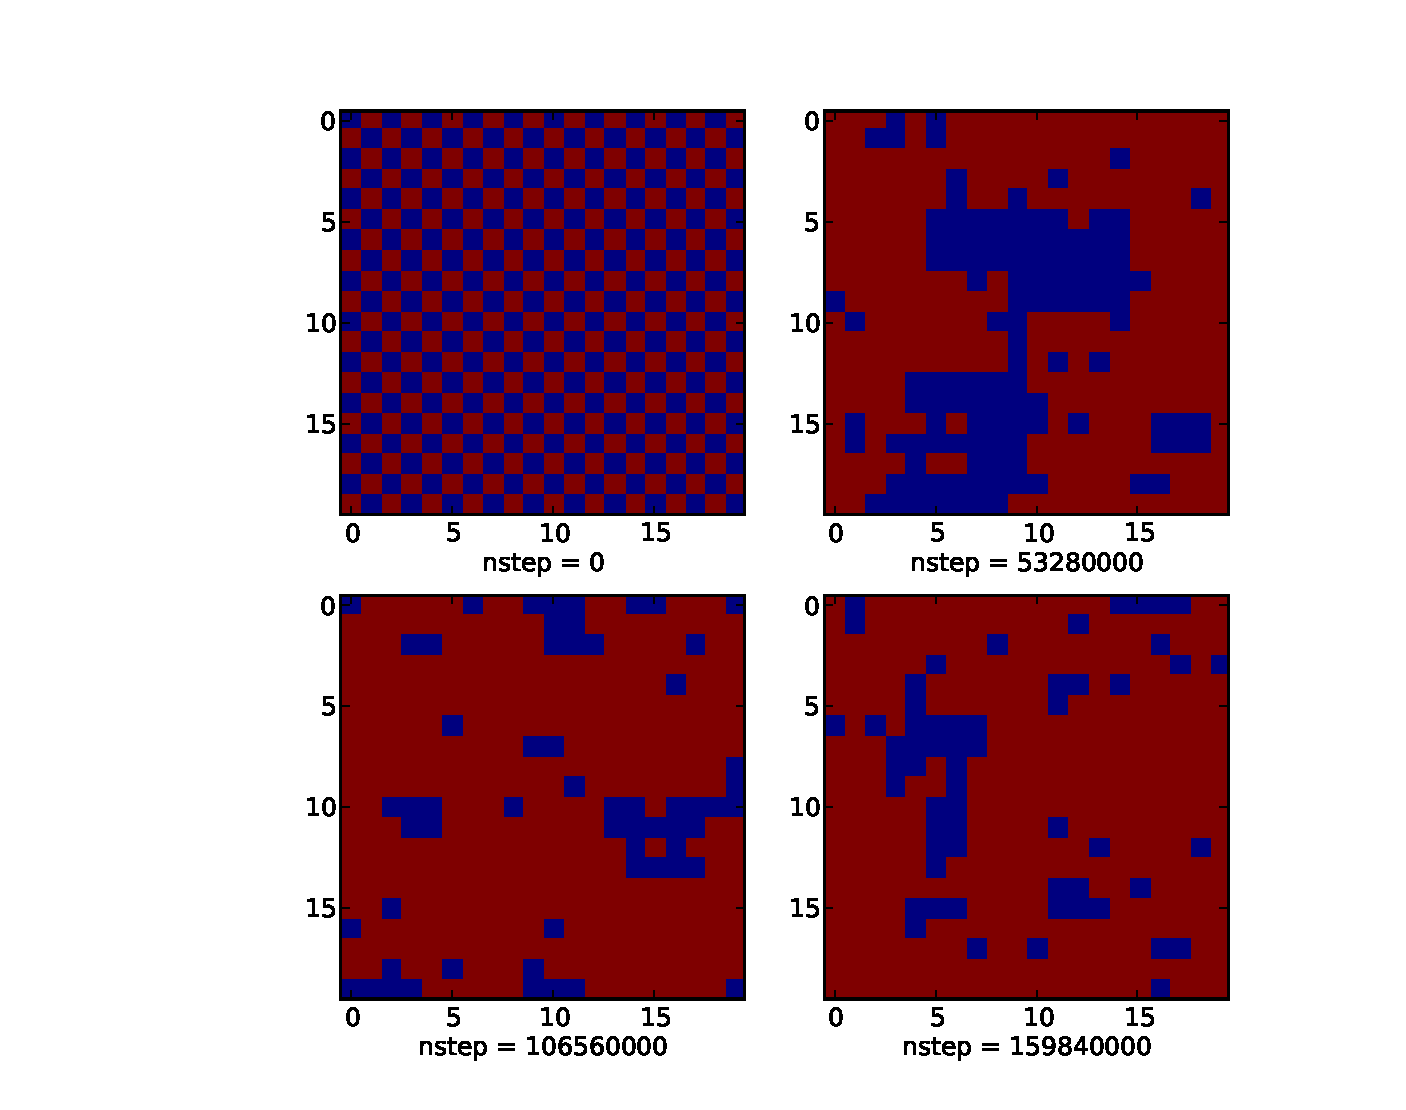
\includegraphics[width=0.53\textwidth]{spin.pdf}
\caption{\label{spin}温度$T=2.4$在不同仿真步时的自旋构型}
\end{figure}
图\ref{energy}为不同温度下系统单个自旋的平均能量, 磁化强度及比热, 磁化率的变化曲线. 从图\ref{energy}中可以看出,
温度在2.2附近发生了相变, 这与二维正方伊辛模型的居里温度$2.26918531\cdots$吻合的很好.
\begin{figure}[!htb]
\centering
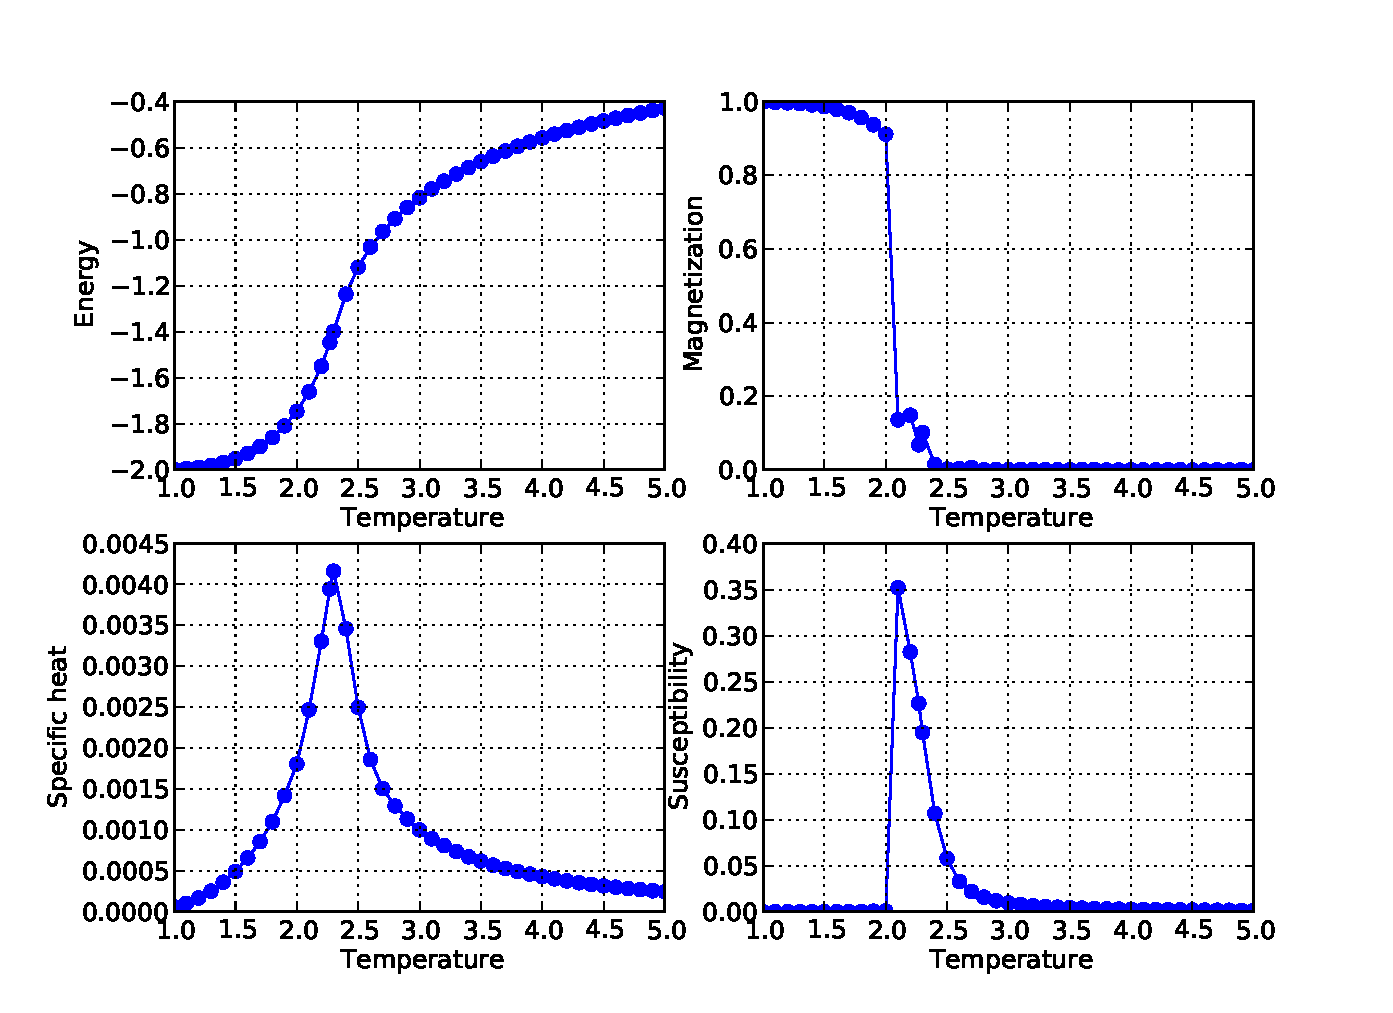
\includegraphics[width=0.6\textwidth]{em.pdf}
\caption{\label{energy}系统单个自旋的平均能量, 磁化强度及比热, 磁化率}
\end{figure}

同时, 蒙特卡罗模拟还可以追踪某一个温度下, 系统能量/磁化强度随时间步长的涨落变化,
图\ref{emchange}是温度为4.0的自旋系统前2400步的能量/磁化强度曲线图. 图\ref{emchange}显示, 系统由初始时刻能量较高的状态, 自发的向能量低的状态迁移, 经过一段时间, 系统能量趋于平稳(上下波动).
\begin{figure}[!htb]
\centering
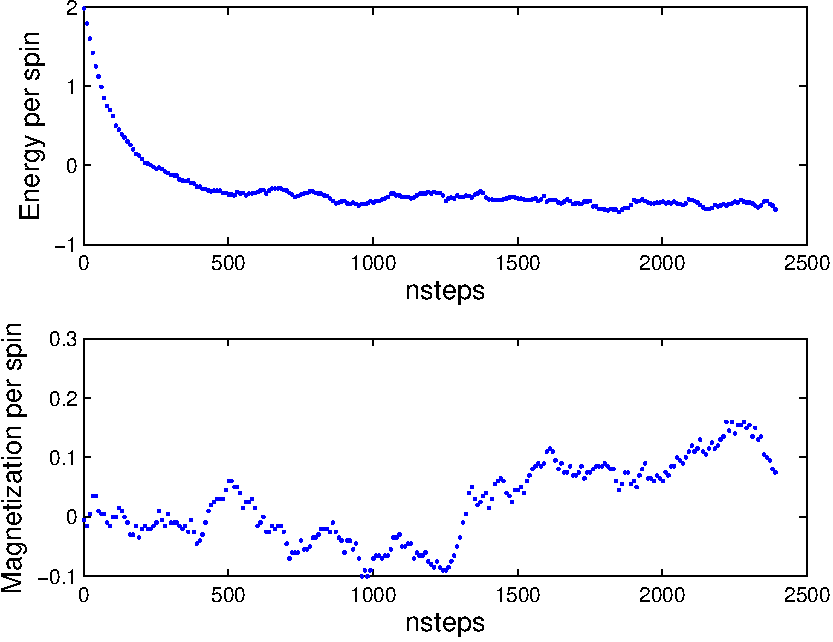
\includegraphics[width=0.55\textwidth]{emchange.pdf}
\caption{\label{emchange}温度T=4.0,checkerboard初始化方式的自旋系统能量/磁化强度随时间步长的变化}
\end{figure}


\section{总结}

本文成功的实现伊辛模型的蒙特卡罗模拟, 验证了二维的伊辛模型确实存在相变的临界温度. 所得到结果与理论或相关文献所给出的计算结果都比较吻合. 同时, 还得到了系统能量/磁化强度的变化曲线图.

另外, 模型和程序经过适当修改, 可推广到更高维数的伊辛模型.

\begin{thebibliography}{99}
\bibitem{wiki} Ising model. \textit{http://en.wikipedia.org/wiki/Ising\_model}.
\bibitem{zhang}张志东. 伊辛模型的研究进展简介. Chinese Journal of Nature. Vol. 30 No. 2
\bibitem{node2}Exact solutions of the Ising model in 1 and 2 dimensions.\\ \textit{http://www.nyu.edu/classes/tuckerman/stat.mech/lectures/lecture\_26/node2.html}
\bibitem{1} \textit{http://www.phy.syr.edu/courses/PHY307.06Fall/LABS/}
\bibitem{2} James P.Sethna. Statistical Mechanics: Entropy, Order Parameters, and Complexity. Oxford University Press. \textit{http://pages.physics.cornell.edu/~sethna/StatMech/}
\bibitem{3} Lisa Larrimore. Monte Carlo Simulation of the 2D Ising Model.

\end{thebibliography}


\newpage
\appendix
\appendixpage
\begin{subappendices}
\section{ising.py}
\begin{python}
"""
ising.py: 2D Monte Carlo Simulation of Ising Model
Zhou Lvwen, zhou.lv.wen@gmail.com
10/02/2011
Physical Simulation: project 02

The model consists of discrete variables called spins that can
be in one of two states. The spins are arranged in a lattice,
and each spin interacts at most with its nearest neighbors.

This program has two output files:

     "SpinArray"     Contains 4 snapshots of the spin lattice at
                     of each temperature run.

     "EnergyMagnet"  Contains six columns: each temperature, the
                     average energy at that temp, the ave energy
                     squared at that temp, the average magnetization
                     at that temp, the ave magnetizaion squared at
                     that temp, the heat capacity, and the
                     susceptibility.
"""

from random import *
from math import *
from sys import *
#########################################################
def initialize(Lx, Ly, ConfigType):
#initialize the spin
   spin = []
   if (ConfigType == 'random'):
      for i in range(0,Lx):
          spin.append([])
          for j in range(0,Ly):
              spin[i] = spin[i] + [choice((-1,1))]
          ##endfor
      ##endfor
   ##endif

   if (ConfigType == 'checkerboard'):
      spinij = 1
      for i in range(0,Lx):
          spin.append([])
          for j in range(0,Ly):
              spin[i] = spin[i] + [-spinij]
              spinij = - spinij
          ##endfor
          spinij = -spinij
      ##endfor
   ##endif

   if (ConfigType == 'interface'):
      for i in range(0,Lx):
          spin.append([])
          for j in range(0,Ly):
              if (i > Lx/2):
                 spin[i] = spin[i] + [ 1]
              else:
                 spin[i] = spin[i] + [-1]
              ##endif
          ##endfor
      ##endfor
   ##endif
   return spin

##end def

#########################################################

def CalculateEnergy(spin, Lx, Ly):
#calculate the initial energy
   E = 0.0
   for i in range(0,Lx):
       for j in range(0,Ly):
           E = E - spin[i][j]*(  \
                                 spin[(i-1)%Lx][j]\
                +spin[i][(j-1)%Ly]               +spin[i][(j+1)%Ly]\
                                +spin[(i+1)%Lx][j] )
       ##endfor
   ##endfor
   return E/2
##end def

#########################################################

def DeltaEnergy(spin, Lx, Ly, i, j):
#calculate the energy difference
    deltaE = 2.0*spin[i][j]*(  \
                               spin[(i-1)%Lx][j]\
                +spin[i][(j-1)%Ly]               +spin[i][(j+1)%Ly]\
                              +spin[(i+1)%Lx][j] )
    return deltaE
##end def

#########################################################

def CalculateMagnet(spin, Lx, Ly):
#calculate the Magnet
   M = 0.0
   for i in range(0,Lx):
       for j in range(0,Ly):
           M = M + spin[i][j]
       ##endfor
   ##endfor
   return M
#end def
#########################################################

Lx = 20; Ly = 20           #number of spins in x and y
N = Lx*Ly                  #total number of spins
Temp = [1+0.1*x for x in range(0,41)] +[2.26918531]
Temp.sort()                #Temperature
MAXITS=N*4000000           #simulation steps
WARM = N*2000000           #equilibrium steps
sample = int(0.333*MAXITS)
data = open("ising.data", 'w')
data.write("Temp"     + "\t" +
           "Energy"   + "\t" +
           "Energy^2" + "\t" +
           "Magnet"   + "\t" +
           "Magnet^2" + "\t" +
           "C_v"      + "\t" +
           "susceptibility"+ "\n")

array = open("ising.spin", 'w')

print("Two-dimensional Ising Model - Metropolis simulation")
print("---------------------------------------------------")
for T in Temp:
    EnergyAve = 0.0
    MagnetAve = 0.0
    Energy2Ave = 0.0
    Magnet2Ave = 0.0
    n = 0
    # Initialize Type = {'random', 'checkerboard', 'interface'}
    spin = initialize(Lx,Ly,'checkerboard')
    Energy = CalculateEnergy(spin,Lx, Ly) # Initialize energy
    print "Running program for T =", T;

    array.write("-----------" + "temperture = " + repr(T)
              + "-----------" + "\n")
    for its in range (0,MAXITS):

        # choose a random spin (i,j)
        i = randint(0,Lx-1)
        j = randint(0,Ly-1)

        deltaE = DeltaEnergy(spin, Lx, Ly, i, j)

        # Accept or refuse the change based on Metropolis criterion
        if (exp(-deltaE/T)>random()):
           spin[i][j] = -spin[i][j]
           Energy +=  deltaE
        ##endif

        Magnet = CalculateMagnet(spin, Lx, Ly)
        if (its >= WARM):
           EnergyAve += Energy/N
           Energy2Ave += (Energy/N)**2
           MagnetAve += Magnet/N
           Magnet2Ave += (Magnet/N)**2
        ##endif
        if (its == n*sample):
           array.write("nsteps = " + repr(its) + "\t" +
                       "Energy = " + repr(Energy/N) + "\n")
           array.write(repr(spin) + "\n")
           n += 1
        ##endif

        if (its%int(0.02*MAXITS)==0):
            stdout.write("-")
            stdout.flush()
    stdout.write(">|" + "\n")
    array.write("\n")
    EnergyAve  /= (MAXITS-WARM)
    Energy2Ave /= (MAXITS-WARM)
    MagnetAve  /= (MAXITS-WARM)
    Magnet2Ave /= (MAXITS-WARM)
    Cv = (Energy2Ave - EnergyAve**2)/T**2
    susceptibility = (Magnet2Ave - MagnetAve**2)/T
    data.write(repr(T)             + "\t" +
               repr(EnergyAve)     + "\t" +
               repr(Energy2Ave)    + "\t" +
               repr(abs(MagnetAve))+ "\t" +
               repr(Magnet2Ave)    + "\t" +
               repr(Cv)            + "\t" +
               repr(susceptibility)+ "\n")
#end for
data.close()
array.close()

print(" M/spin and E/spin values written in ising.data")
print(" spin array written in ising.spin")
print(" Done ... Performing production steps ...")
\end{python}

\section{isingplot.py}
\begin{python}
"""
isingplot.py: import ising.data and plot figures
Zhou Lvwen, zhou.lv.wen@gmail.com
10/02/2011
Physical Simulation: project 02
"""

from matplotlib.pyplot import *
import sys
import string

def getNumArrFromFile(filename):
    arr = []
    a_file = open(filename,mode='r')
    filestr = a_file.readline()
    filestr = a_file.readline()
    n = 0
    while filestr:
       arr.append([])
       linearr = filestr.split('\n')
       for line in linearr:
           numarr = line.split()
           for numstr in numarr:
               arr[n] = arr[n] +[string.atof(numstr)]
       n += 1
       filestr = a_file.readline()
    return arr
#end def

data = getNumArrFromFile('ising.data')

T = []
Energy= []
Energy2 = []
Magnet = []
Magnet2 = []
Cv = []
susceptibility = []
for i in range(0,len(data)):
    T += [data[i][0]]
    Energy += [data[i][1]]
    Energy2 += [data[i][2]]
    Magnet += [data[i][3]]
    Magnet2 += [data[i][4]]
    Cv += [data[i][5]]
    susceptibility += [data[i][6]]

subplot(221)
plot(T,Energy,'.-', markersize = 13)
grid()
xlabel('Temperature')
ylabel('Energy')

subplot(222)
plot(T,Magnet,'.-', markersize = 13)
grid()
xlabel('Temperature')
ylabel('Magnetization')

subplot(223)
plot(T,Cv,'.-', markersize = 13)
grid()
xlabel('Temperature')
ylabel('Specific heat')

subplot(224)
plot(T,susceptibility,'.-', markersize = 13)
grid()
xlabel('Temperature')
ylabel('Susceptibility')
show()
\end{python}
\end{subappendices}

\end{document}
